\documentclass{standalone}
\usepackage{amsmath} 
\usepackage{amssymb} 
\usepackage{tikz}
\usetikzlibrary{arrows,calc,shapes,fit,decorations.text}


\begin{document}
\newsavebox{\event}
\savebox{\event}{
  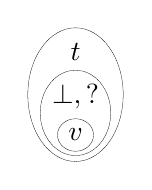
\begin{tikzpicture}[el/.style={shape=ellipse, draw, ultra thin},]
    \node [el, draw, inner sep=2pt] (v) {$v$};
    \node [anchor=south] (e) at (v.north) {$\bot, ?$};
    \node [el, fit=(v)(e), inner sep=-3pt] (ve) {};   
    \node [anchor=west,inner sep=2pt] (d1) at (ve.east) {};
    \node [anchor=east,inner sep=2pt] (d2) at (ve.west) {};
    \node [anchor=south] (t) at (ve.north) {$t$};
    \node [el, fit=(ve)(t)(d1)(d2), inner sep=-5pt] {}; 
  \end{tikzpicture}
}
\newsavebox{\extvalue}
\savebox{\extvalue}{
  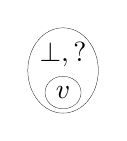
\begin{tikzpicture}[el/.style={shape=ellipse, draw, ultra thin},]
    \node [el, draw, inner sep=2pt] (v) {$v$};
    \node [anchor=south] (e) at (v.north) {$\bot, ?$};
    \node [el, fit=(v)(e), inner sep=-3pt] (ve) {};   
  \end{tikzpicture}
}

\begin{tikzpicture}[scale=0.8, every node/.style={scale=0.8}]
  \node (e0) at (-1,5) {$\cdots$};
  \node (e1) at (0,5) {\usebox{\event}};
  \node (e2) at (1.5,5) {\usebox{\event}};
  \node (e3) at (3,5) {\usebox{\event}};

  \path[draw]  (e0.west) |- (e1.north west) -- (e3.north east) --++(2,-2) --++(.5,.5) --++(0,-2) 
              coordinate (synchl) {}; 
  \path[draw] (synchl) --++(-2,0) --++(.5, .5) -- (e3.south east) -- (e1.south west) -| (e0.west);
  \node[yshift=-5pt, anchor=north] at (e2.south) {\emph{Signal}};

  \def\myshift#1{\raisebox{-3ex}}
  \draw[postaction={decorate, decoration={
      text along path,
      text align=right,
      text={|\sffamily\LARGE\myshift|Synchronization layer}}}
  ] (synchl) arc (135:80:10cm); 
  \draw[postaction={decorate, decoration={
      text along path,
      text align=center, reverse path, raise={2.5ex},
      text={|\sffamily\it|Process}}}
  ] (synchl) arc (135:180:10cm) coordinate (synchend);
  \node (mocd) at ($(synchl)+(1,-1)$) {\usebox{\event}};
  \node[anchor=west, text width=5em, font=\footnotesize] at (mocd.north east) {operates on events};
  \node[anchor=north , text width=8em, yshift=-30pt, xshift=-18pt, font=\footnotesize] at (mocd.south west) {Abstracts: \\ 
    $\bullet$ MoC semantics \\ 
    $\bullet$ time behavior \\ 
    $\bullet$ synchronization};

   \draw[postaction={decorate, decoration={
      text along path,
      text align=right,
      text={|\sffamily\LARGE\myshift|Behavior layer}}}
  ] ($(synchend)+(3cm,0)$) arc (180:80:7.45cm); 
  \node (behd) at ($(mocd)+(2,-2)$) {\usebox{\extvalue}};
  \node[anchor=west, text width=5.5em, font=\footnotesize] at (behd.north east) {operates on extended values};
  \node[anchor=north , text width=8em, yshift=-15pt, xshift=-6pt, font=\footnotesize] at (behd.south west) {Abstracts: \\ 
    $\bullet$ extended value semantics \\ 
    $\bullet$ behavior in case of special events};

   \draw[postaction={decorate, decoration={
      text along path,
      text align=right,
      text={|\sffamily\LARGE\myshift|Function layer}}}
  ] ($(synchend)+(6cm,0)$) arc (180:80:4.9cm); 
  \node [shape=ellipse, draw, ultra thin, inner sep=2pt] (fcd) at ($(behd)+(2,-2)$) {$v$};
  \node[anchor=west, text width=5.5em, xshift=5pt, font=\footnotesize] at (fcd.east) {operates on values};
  \node[anchor=north , text width=8em, yshift=-15pt, font=\footnotesize] at (fcd.south west) {Abstracts nothing};
\end{tikzpicture}

\end{document}
%%% Local Variables:
%%% mode: latex
%%% TeX-master: t
%%% End:
